\section{Complex networks}

Graph theory is a well established area of mathematics. More recently, other areas from physics to economics, sociology to ecology have found that the structures and properties of graphs give a powerful and practical method of representing systems of interest to them. This new focus on what might have been called applied graph theory is what is now mostly know as network science. One of the interesting aspects of network science is that it deals with structures that are non-regular (not lattice-like) but also not purely random. These heterogeneous patterns of connections have implications for the study of complex systems (systems of entities with non-trivial sets of typically non-linear interactions) and hence networks often get referred to as complex networks. The Complex part of the name is really a bit redundant, but it sounds good and is commonly used, so we'll stick with it.

\subsection{An introduction to graph theory \& networks}

A network or \emph{graph} is a collection of \emph{vertices} (nodes) $V=\{v_i\}$ and \emph{edges} (links) $E=\{e_{ij}\}$ which we denote $G= G(V,E)$.

If we consider the edge $e_{ij}$, between vertices $v_i$ and $v_j$ to be distinct from $e_{ji}$ then we say that the edge is \emph{directed}. A graph is directed if all its edges are directed. A \emph{simple graph} is a network (possibly directed) where there is a unique (directed) edge between connected pairs of nodes. A \emph{multigraph} allows for the possibility of multiple edges edges between the same nodes. We will mostly only consider simple graphs, though much of what we'll present also holds for multigraphs, with a slight adjustment. 

The \emph{density} of a graph is the number of edges present in the graph divided by the number of possible edges. For an undirected simple graph with $|V|=n$ nodes, the density is given by
$$
	\rho = \frac{|E|}{\frac12 n(n-1)},
$$
where $|E|$ is the number of edges and where the factor of $\frac12$ comes from the fact that the edges are undirected so $e_{ij}=e_{ji}$. 

The \emph{degree} of a node in a network, often denoted $k$ or $k_i$ for the degree of node $i$ is the number of edges that connect to that node. In the case of a directed network we have both \emph{in-degree} and \emph{out-degree}, the number of incoming and outgoing links, respectively.

The \emph{component} of a graph to which a vertex belongs is the set of vertices that can be reached from it by paths running along the edges of the graph. A node in a directed graph has both an \emph{in-component} and an \emph{out-component} corresponding to the nodes that it can be reached from and the nodes that can be reached from it. A graph need not consist of only a single component, though some properties are ambiguously defined when it does not.

The \emph{geodesic path} between a pair of nodes is the shortest path through the network that connects them. The shortest path need not be unique and for a directed network the shortest path can differ depending on direction.
It is sometimes interesting to look at the \emph{average shortest path} for a graph. That is the average over all possible shortest paths in the graph, computed for each pair of nodes. 

The notation $e_{ij}$ for the edges of a network suggests that we can represent a network as a matrix. If we let the rows and columns of the matrix represent the vertices of the network, then the non-zero entries of the matrix represent edges between pairs of vertices. We call such a network the \emph{adjacency matrix} of the graph. The values of the non-zero entries can be used to denote \emph{edge weights} of a \emph{weighted graph}.

Many real-world networks consist of nodes of different types, with connection only between nodes of certain types. The simplest example of this is a \emph{bipartite network} (also known as a \emph{two-mode network}): a network of two types of vertices $V=\{v_i\}$ and $U=\{u_j\}$ where the edges only connect nodes of type $v$ to nodes of type $u$. For example, a publication network where $V$ represents authors and $U$ their publications.  (More generally, the two node types are often referred to as agents and artifacts.) Edges link authors to their publications but not publications to publications, nor authors to authors. In order to obtain a co-authorship network from this publication network it would be necessary to calculate the \emph{unipartite} or \emph{one-mode projection} of the bipartite network.


\subsection{Real-world networks: some examples}

{\bf Social networks:} 

A social network is a set of people or groups with some pattern of contacts or interactions between them. They include such diverse examples as friendship networks of dolphins and interactions between characters in works of fiction, through to more traditional networks such as friendships between individuals, either in real life, or on Facebook, employment networks, and business relationships between companies.

Some of these networks, like the business relationships are best viewed as undirected networks, while others, like real-life friendship networks are directed. Friendship networks lend their name to an interesting feature of networks: the so called \emph{friendship paradox} which states that your friends will typically have more friends than you do. This arises from the fact that like many other real-world networks, friendship networks have a heavy-tailed degree distribution so picking a random node and following an edge from it is likely to lead you to a node with higher degree than the starting node.

\emph{Contact networks} are one important example of social networks. These are networks of when people are in close enough proximity to allow for a disease to spread between them. (Close enough obviously depends on the type of disease.) Contact networks play an important role in modeling of disease contagion --- for example the recent Ebola outbreak in West Africa was successfully modeled using contact networks and this played an important role in managing the epidemic.



{\bf Information networks:}

These could equally be called knowledge networks. Examples include the publication networks mentioned earlier (bipartite, undirected), citation networks (directed) whether as citations of publications or of patents, and the World Wide Web (directed). (Note --- the WWW should not be confused with the internet; one is a collection of electronic documents that can link to one another, the other is a collection of computers and switches connected by cables.) Preference networks are another example of information networks that are often used in real-world applications. Examples include networks of people linked to their Netflix viewings, or their Amazon purchases. Identifying patterns in such networks and predicting likely new links is a highly active area of both academic and commercial interest.


{\bf Technological \& infrastructure networks:} 

These are networks with physical links between nodes. Examples include the internet (undirected); electricity grids (partly directed) perhaps also including the computers that control the grid; road, rail, shipping, or air transport networks; and electronic circuits. 


{\bf Biological networks:} 

These networks span multiple scales, from networks of interactions between proteins and their metabolites, or genes and proteins (both directed) that are used amongst other things, in the study of disease through to networks of interactions between species. The latter includes food webs (directed) and mutualistic networks like pollination networks (bipartite, directed). Neural networks are another example that is an active area of study; the complete neural network (282 neurons) is known for the nematode C. Elegans. Studying bigger brains, however, requires bigger brains. Though not entirely biological, I'll include in this class a couple of examples of physical networks. These are networks linking free energy minima of glasses via the saddle points on the energy surface that they sit on and networks linking confirmations of polymers when they can transition between a pair of structures. 


\subsection{Properties of networks}

{\bf Small world effect:}

One of the best know network properties is the \emph{small world effect}. This gets it name from a famous experiment in the 1960s by the sociologist Stanley Milgram. In the experiment, letters were passed from person to person until they reached a designated target person. Milgram found that it took on average only about six hops for the letters to reach their destination leading to the so called \emph{six degrees of separation} phenomenon. This small world effect is an example of how particular network structures can provide short paths through the network connecting most pairs of nodes. 

The mean geodesic path length for an undirected network is given by
$$
	L =\frac{1}{\frac12 n(n-1)}\sum_{i\geq j} d_{ij}
$$
where $d_{ij}$ is the geodesic distance between $v_i$ and $v_j$. In the case of disconnected networks, one must make a choice about how to count the contribution of pairs of nodes that are not connected. The Facebook friendship network is one of the best examples of a small world network. Despite having around 1 billion nodes and 100 billion links (i.e. a mean degree of 100) the mean geodesic distance for the Facebook network is only around four.

{\bf Transitivity/clustering:}

In mathematics, a set with a relationship $\sim$ is transitive if $a \sim b,~b\sim c \implies a \sim c$. In the context of networks the relationship means "is connected to". If a network is entirely transitive, then it would consist of totally connected components. More interesting is to measure how close a network is to being transitive by looking at how much clustering it has.

The \emph{global clustering coefficient} for a network is defined as
$$
	C=\frac{3\times\text{\# of triangles}}{\text{\# number of connected triples}}
$$
where a connected triple is a vertex with connections to two other vertices.

It is sometime interesting to look at how the clustery-ness of a network varies over the network, perhaps to study how clustering depends on some node property. To look at this, we use the \emph{local clustering coefficient} for a vertex $v_i$:
$$
	C_i = \frac{\text{\# triangle connected to }v_i}{\text{\# triples centered on }v_i}.
$$
Clearly, $C = \frac{1}{N}\sum_{i=1}^NC_i$.

Now that we've defined the clustering coefficient, we can look a little closer at the small world property.
If we start with a completely regular network (figure \ref{fig1}a) where each node has the same degree $k$ and is connected to its $k$ nearest neighbours we will have a high clustering coefficient, but a relatively long mena geodesic path. If we start to introduce random re-wirings of the network, with probability $p$, by either switching an end of an existing edge (figure \ref{fig1}b) or by introducing new random links (figure \ref{fig1}c), then we find that the mean geodesic path length drops quickly, while the mean clustering coefficient remains close to its original value as the re-wiring probability $p$ increases --- see figure \ref{fig2}. This means that while the long-range connections rapidly reduce the \emph{global} mean path geodesic length, any change to the \emph{local} structure is barely perceptible.

\begin{figure}
	\begin{center}
		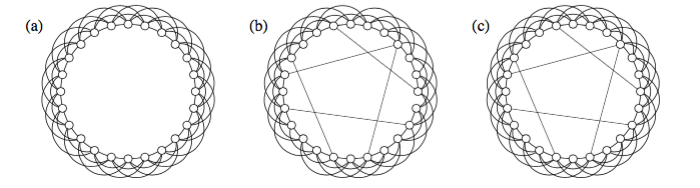
\includegraphics[width = 12cm]{regularNW.png}
	\end{center}
	\caption{}
	\label{fig1}
\end{figure}

\begin{figure}
	\begin{center}
		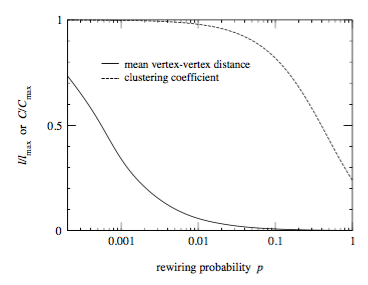
\includegraphics[width = 8cm]{smallWorld.png}
	\end{center}
	\caption{Mean geodesic path length (solid line) and mean clustering coefficient (dashed line) as a function of the rewiring probability $p$, and measured relative to their maximum value, i.e. with no re-wiring.}
	\label{fig2}
\end{figure}


{\bf Degree distribution:}

The degree $k$ of a vertex is the number of edges that connect to that vertex. We write $p_k$ for the fraction of nodes in a network that have degree $k$, this is also the probability that a randomly selected node has degree $k$. One of the interesting properties of real-world networks is the degree distribution --- the histogram of $p_k$ as a function of $k$. For a network with uniformly random connections between nodes, the degree distribution is Poisson. This is not the case for most real-world networks --- these tend to have degree distributions that are highly right-skewed. In particular, many real-world networks tend to have a \emph{heavy-tail} --- a probability distribution that has a non-negligible probability of getting values much greater than the mean. In fact, the mean (and higher order moments like the variance) may not even be well defined for all heavy-tailed distributions.  Of particular interest is the case where the degree distribution is a \emph{power-law} or \emph{scale-free}. That is
$$
 p_k \sim k^{-\gamma}.
$$

Such degree distributions show up surprisingly often in real world networks: the WWW, the internet, metabolic networks, telephone call networks, and sexual contact networks. Power law degree distributions also arise from one of the most popular models for generating networks --- we'll see more on this later.

An alternative (i.e. non-power-law) distribution that is still heavy-tailed is the \emph{exponential distribution}
$$
	p_k\sim\exp(-k/\kappa).
$$

Power-law and exponential distributions are easily identified in data: they give a straight line on log-log and semi-log axes, respectively.

\subsection{Probability Generating Functions \& Networks}
The probability generating functions that we introduced at the start of the course give a useful way of calculating network properties from their degree distributions. For example, if $G_0(x) = \sum_{k=0}^\infty p_kx^k$ is the PGF for the degree distribution of a network, then the first moment of the PGF gives the average degree, $\langle k \rangle$, of the network, according to
$$
	G_{0}'(x) = \sum_{k}kp_{k}x^{k-1},
$$
and
$$
	G_{0}'(1) = \sum_{k}kp_{k} = \langle k \rangle.
$$	

Another important property is the degree distribution of first neighbours. The reasoning is as follows: by selecting a link at random, and following it until reaching a node, we will find that the node has, let's say, degree $k$. The probability with which we will reach such a node is proportional to its degree ($\propto kp_{k}$). The normalized distribution is given by
$$
	\dfrac{\sum kp_{k}x^{k}}{\sum_{k}kp_{k}} = x \dfrac{\sum kp_{k}x^{k-1}}{\langle k \rangle} = \dfrac{x}{\langle k \rangle}G_{0}'(x).
$$

Then, by following each one of the $k$ edges of a randomly chosen node of degree $k$, we have the distribution of the remaining outgoing edges of the $k$ first neighbours of that node generated by the function 
$$
	G_{1}(x) = \dfrac{\sum_{k}kp_{k}(k)x^{k-1}}{\langle k \rangle} = \dfrac{1}{\langle k \rangle}G_{0}'(x)
$$
Note that because we are following the edges of a randomly chosen node, the distribution of the remaining edges of the first neighbours do not count the edge by which we arrived at that neighbour. That is why we get rid of one power of $x$ in the equation for $G_{1}(x)$.

From that, it is not hard to find a new PGF for the number of second neighbours of nodes in a network. 
$$\sum_k p_k (G_1(x))^k $$ 
where 
$$G_1(x) = \frac{G_{0}'(x)}{G_{0}'(1)}$$ 
This, in turn, is close to the PGF for the degree distribution of the projection of a bipartite network, since the second neighbours of a bipartite network are the neighbours of its projection.

\subsection{Network growth models}
It is one thing to be able to produce a network, fully formed, with a particular set of properties. It is quite another to prescribe a process that is able to grow, or generate, a network with those same properties.

One popular generative network model is the \emph{preferential attachment plus growth model} (PAGP model), also known as the Barabasi and Albert or BA model.

As the name suggests, at each time step, the PAPG model adds a node with degree $m$. Each of the edges of the new node attaches itself to a node in the existing network with a probability that is proportionate to the degree of the existing nodes. The edges in this model are undirected and once and edge is attached to a node, there is no re-wiring. It isn't too hard to prove that the PAPG model generates graphs with a power law degree distribution with $p_k \sim k^{-3}$. The fact that the power law exponent is fixed is unfortunate, though generalisation of the PAPG model allow for different exponents. It is also not hard to see that the PAPG model only produces connected graphs. This limits its applicability to some real world networks. Even though the PAPG model manages to grow networks that reproduce some real-world features (the power-law degree distribution), it does so in a way that may not match up with the growth processes of those real-world networks. For example the highest degree nodes of the PAPG model are the oldest nodes --- this is not the case with networks such as the WWW to which the PAPG model might be applied.


\subsection{Exponential random graph models}
Given a particular empirical network one often wants to create models of networks with similar observable properties. These observables might be any of the properties mention so far (or many others) such as mean clustering or a particular degree distribution. One approach is to consider the empirical network as one example of a network from an ensemble of networks that have been generated by the same underlying model. Exponential random graph models (ERGMs) provide a way to study the properties of such models by employing methods that come directly from the statistical mechanics that we have seen so far.

Consider a set $\mathcal{G}$ of graphs and a collection of observables $\{X_i\},~~i=1,2,\ldots,r$ for which we have measured expected values $\langle X_i\rangle$. It will often turn out that we only have a single measurement of these values. (Here we'll assume that the graphs in $\mathcal{G}$ are simple graphs, but the same approach works for many other possibilities.) Given a specific graph $G\in\mathcal{G}$ we want $P(G)$ the probability of finding that graph to be commensurate with the expected values of each of the graph observables $\{X_i\}$. Just like for statistical  mechanics, this is an under-determined problem: the number of degrees of freedom for the definition of $P(G)$ is much smaller than the number of constraints from the observables. However, as we know from statistical mechanics, the best approach is to pick the solution that maximises the Gibbs entropy
$$
	S= -\sum_{G\in\mathcal{G}}P(G)\ln P(G),
$$
subject to the constraints
$$
	\sum_G P(G)X_i(G) = \langle X_i\rangle
$$
and the normalization condition
$$
	\sum_G P(G) =1.
$$

To do this, we introduce the Lagrange multipliers $\alpha$ and $\theta_i$ and solve
$$
	\frac{\partial}{\partial P(G)}\left[S + \alpha \left(1-\sum_G P(G)\right) + \sum_i \theta_i \left(\langle X_i \rangle - \sum_G P(G)X_i(G)\right) \right] = 0
$$
for all graphs $G$.

This gives
$$
	\ln P(G) +1 +\alpha +\sum_i\theta_iX_i(G) = 0.
$$

We can rearrange this to get
$$
	P(G) = \frac{\exp(-H(G))}{Z},
$$
where $H(G) = \sum_i\theta_iX_i(G)$ is known as the graph Hamiltonian and $Z = \exp(\alpha+1)$ is the partition function. The requirement that $Z$ be a normalising factor requires that $\exp(\alpha+1) = \exp(-H(G))$.


\subsection{Recommended reading}
There are several good books on complex networks, including \emph{Lectures on Complex Networks} by S.N. Dorogovtsev and \emph{The Structure of Complex Networks} by E. Estrada, but some of the best content is in the form of journal survey articles. My picks are the two by M.E.J. Newman: \emph{The Structure and Function of Complex Networks} and, joint with J. Park \emph{Statistical Mechanics of Networks}. I used both of these extensively in writing this section. Also good is \emph{Statistical Mechanics of Complex Networks} by R. Albert and A.-L. Barabasi. For a good survey of generative models for power law distributions, see the survey article by Mitzenmacher.

